%!TEX program = xelatex
%% Copyright (C) 2025 傅祉珏
%% 
%% 此文件是《Homework2 基于PCA/LDA和KNN的人脸识别》的LaTeX源码,依据AGPLv3许可证发布。
%% 完整许可证文本见项目根目录LICENSE文件,附加限制条款见ADDITIONAL_TERMS.md。
%% 
%% 禁止商业用途,学术使用需保留本声明。
%% 源码仓库:https://github.com/Billiefu/YatPR

% SPDX-FileCopyrightText: 2025 傅祉珏
% SPDX-License-Identifier: AGPL-3.0-or-later
% SPDX-Additional-Clauses: see ADDITIONAL_TERMS.md

\documentclass[a4paper, utf8]{ctexart}
\usepackage[fontset=Fandol]{ctex}
\usepackage{draftwatermark}
\usepackage{anyfontsize}
\usepackage{indentfirst}
\usepackage{subcaption}
\usepackage{amsfonts}
\usepackage{enumitem}
\usepackage{tabularx}
\usepackage{fancyhdr}
\usepackage{geometry}
\usepackage{graphicx}
\usepackage{abstract}
\usepackage{amsmath}
\usepackage{lipsum}

% 设置页面间距
\geometry{a4paper,left=31mm,right=31mm,top=25mm,bottom=25mm}
% 章节标题左对齐
\CTEXsetup[format={\Large \bfseries}]{section}
% 段首缩进2字符
\setlength{\parindent}{2em}
% 设置页眉及页脚 页码
\pagestyle{fancy}
\fancyhf{}
\fancyhead[C]{}
\fancyhead[L]{Homework2 \ \  基于 PCA/LDA 和 KNN 的人脸识别}
\fancyhead[R]{21307210 \ \  傅祉珏}
\fancyfoot[C]{\thepage}
\fancyfoot[L,R]{}

% 使宋体可加粗
\setCJKfamilyfont{zhsong}[AutoFakeBold = {2.17}]{SimSun}
\renewcommand*{\songti}{\CJKfamily{zhsong}}

% 定义标题 作者及单位信息
\title{\songti \Large \textbf{Homework2 \quad 基于 PCA/LDA 和 KNN 的人脸识别}}
\author{\fangsong 21307210 \ \  傅祉珏}
\date{\fangsong 中山大学计算机学院 \ \  广东广州 \ \  510006}

% 版权信息水印
\SetWatermarkText{Copyright\ \copyright\ 2025\ 傅祉珏}
\SetWatermarkScale{0.4}
\SetWatermarkAngle{45}
\SetWatermarkColor[gray]{0.8}

\begin{document}

	\begin{titlepage}
		\centering
		\rule{\textwidth}{1pt}
		\vspace{0.02\textheight}
		
		{\LARGE \kaishu 模式识别 \quad SYSU\ CSE\ 2024-2 \quad 课程作业}
		
		\vspace{0.02\textheight}
		
		{\Huge \songti \bfseries Homework2 \ \  基于 PCA/LDA 和 KNN 的人脸识别}
		
		\vspace{0.025\textheight}
		\rule{0.83\textwidth}{0.4pt}
		\vspace{0.05\textheight} 
		\begin{figure}[htbp]
			\centering
			\includegraphics[width=8cm, height=8cm]{./figure/计院院徽.jpg}
		\end{figure}
		
		\vspace{0.04\textheight} 
		{\Large 课程编号:\textsc{DCS299}}
		
		\vspace{0.025\textheight} 
		{\Large 实验人员姓名:\textsc{傅祉珏}}
		
		\vspace{0.025\textheight} 
		{\Large 实验人员学号:\textsc{21307210}}
		
		\vspace{0.025\textheight} 
		{\Large 指导教师姓名及职称:\textsc{马锦华\ 副教授}}
		
		\vspace{0.025\textheight} 
		{\Large 项目截止时间:\textsc{2025年4月27日}}
		
		\vspace{0.05\textheight} 
		\vfill
		
		{\large \today}
		\vspace{0.1\textheight}
		\rule{\textwidth}{1pt}
	\end{titlepage}
	\let\cleardoublepage\clearpage
	
	\maketitle
	
	\renewcommand{\abstractname}{\large \textbf{摘要}}
	\begin{abstract}
		在人脸识别任务中,如何从高维图像中提取具有判别性的特征并实现高效分类,一直是模式识别与计算机视觉领域的重要课题。本文围绕经典降维方法主成分分析(PCA)与线性判别分析(LDA),设计并实现了一个完整的人脸识别实验系统。实验在 Yale 人脸数据集上,分别采用 PCA 和 LDA 对人脸图像进行特征提取,并结合 K 最近邻(KNN)与支持向量机(SVM)两类分类器,系统比较不同组合方案在识别准确率方面的差异。实验结果表明,在使用 KNN 分类器时,PCA 降维效果优于 LDA,而在使用 SVM 分类器时,LDA 展现出更强的分类性能,分别达到 93.33\% 的最高识别率。这一结果说明,不同降维方式在不同分类模型中的适配性存在显著差异,具有互补特性。最终,本实验验证了降维方法与分类策略之间的协同作用,并为构建高效且可解释的轻量级人脸识别系统提供了实践基础与对比分析框架。
		
		\noindent{\textbf{\heiti 关键词:}PCA;LDA;KNN;SVM;人脸识别;特征降维。}
	\end{abstract}
	
	\section{引言}
	
	在人脸识别等计算机视觉任务中,如何从高维图像数据中提取具有判别力的特征并实现高效分类,一直是研究的核心问题。人脸识别在现实生活中的应用十分广泛,从手机解锁、门禁系统到公共安全监控,其在保障个人信息安全和社会治安方面发挥着重要作用。随着深度学习的发展,人脸识别系统在性能上取得了巨大突破,但特征提取和分类的基本思想仍然根植于诸如主成分分析(PCA)与线性判别分析(LDA)等经典模式识别方法之中。因此,深入理解和掌握这些降维与分类技术,对于构建更高效、可解释、轻量级的人脸识别系统具有重要意义。
	
	然而,在人脸识别任务中,原始图像数据往往维度极高,不仅增加了计算开销,也容易引发“维度灾难”,导致分类性能下降。传统的降维方法如 PCA 和 LDA,虽然在数据压缩与特征提取方面表现优异,但在实际应用中仍面临诸如样本数量不足、类间差异模糊等问题\cite{hfd,pcavslda}。此外,分类器的选择也对识别效果有显著影响,特别是在小样本学习场景下,如何设计鲁棒、简洁且有效的分类方法成为研究重点\cite{hfd}。
	
	本次作业\textbf{实现了基于 PCA 与 LDA 的人脸图像降维算法,并结合 K 最近邻(KNN)分类器完成识别任务。}实验中不依赖库函数接口,全面锻炼对底层算法的理解与实现能力。PCA 作为无监督降维方法,通过最大化样本的投影方差来提取主成分,有效保留图像的全局结构特征;LDA 则利用类别标签信息,通过最大化类间散度与最小化类内散度的比值,实现更具判别力的特征投影。KNN 分类器作为一种基于距离的非参数方法,简洁直观,适用于小样本场景中的分类任务,能较好地反映降维后特征的分布规律。本次实验将对上述方法进行系统实现与实验评估,为深入理解经典机器学习技术在人脸识别中的应用打下坚实基础。
	
	\section{相关工作}
	
	人脸识别作为计算机视觉领域的重要研究方向之一,在身份验证、公共安全、智能交互等场景中具有广泛的实际应用价值。其关键前提在人脸检测与表征,随后借助有效的分类方法实现身份判别。在众多的人脸识别技术中,基于降维的特征提取方法与分类器的结合是经典且实用的方案。为此,大量研究工作聚焦于提升人脸检测、特征降维与分类的性能与适应性。
	
	早期的人脸检测方法多基于颜色空间建模和结构特征分析,如 YCgCr 及 YCbCr 色彩空间被广泛应用于肤色建模,Ghanzali 等提出了基于 YCgCr 色彩空间的创新人脸检测方法,在复杂背景中表现出较好的鲁棒性\cite{chfd2}。De Dios 和 Phung 等学者也分别从不同的色彩模型出发,构建了适应不同肤色、光照条件和背景干扰的检测机制\cite{chfd1, chfd3}。近年来,Alashbi 等进一步提出在严重遮挡与非约束环境下的人脸检测框架,有效提升了系统的鲁棒性与适应性\cite{mhfd1}。
	
	\begin{figure}[htbp]
		\centering
		\begin{subfigure}{.35\textwidth}
			\centering
			\includegraphics[height=.12\textheight]{./figure/color1.png}
		\end{subfigure}
		\begin{subfigure}{.25\textwidth}
			\centering
			\includegraphics[height=.12\textheight]{./figure/color2.png}
		\end{subfigure}
		\begin{subfigure}{.35\textwidth}
			\centering
			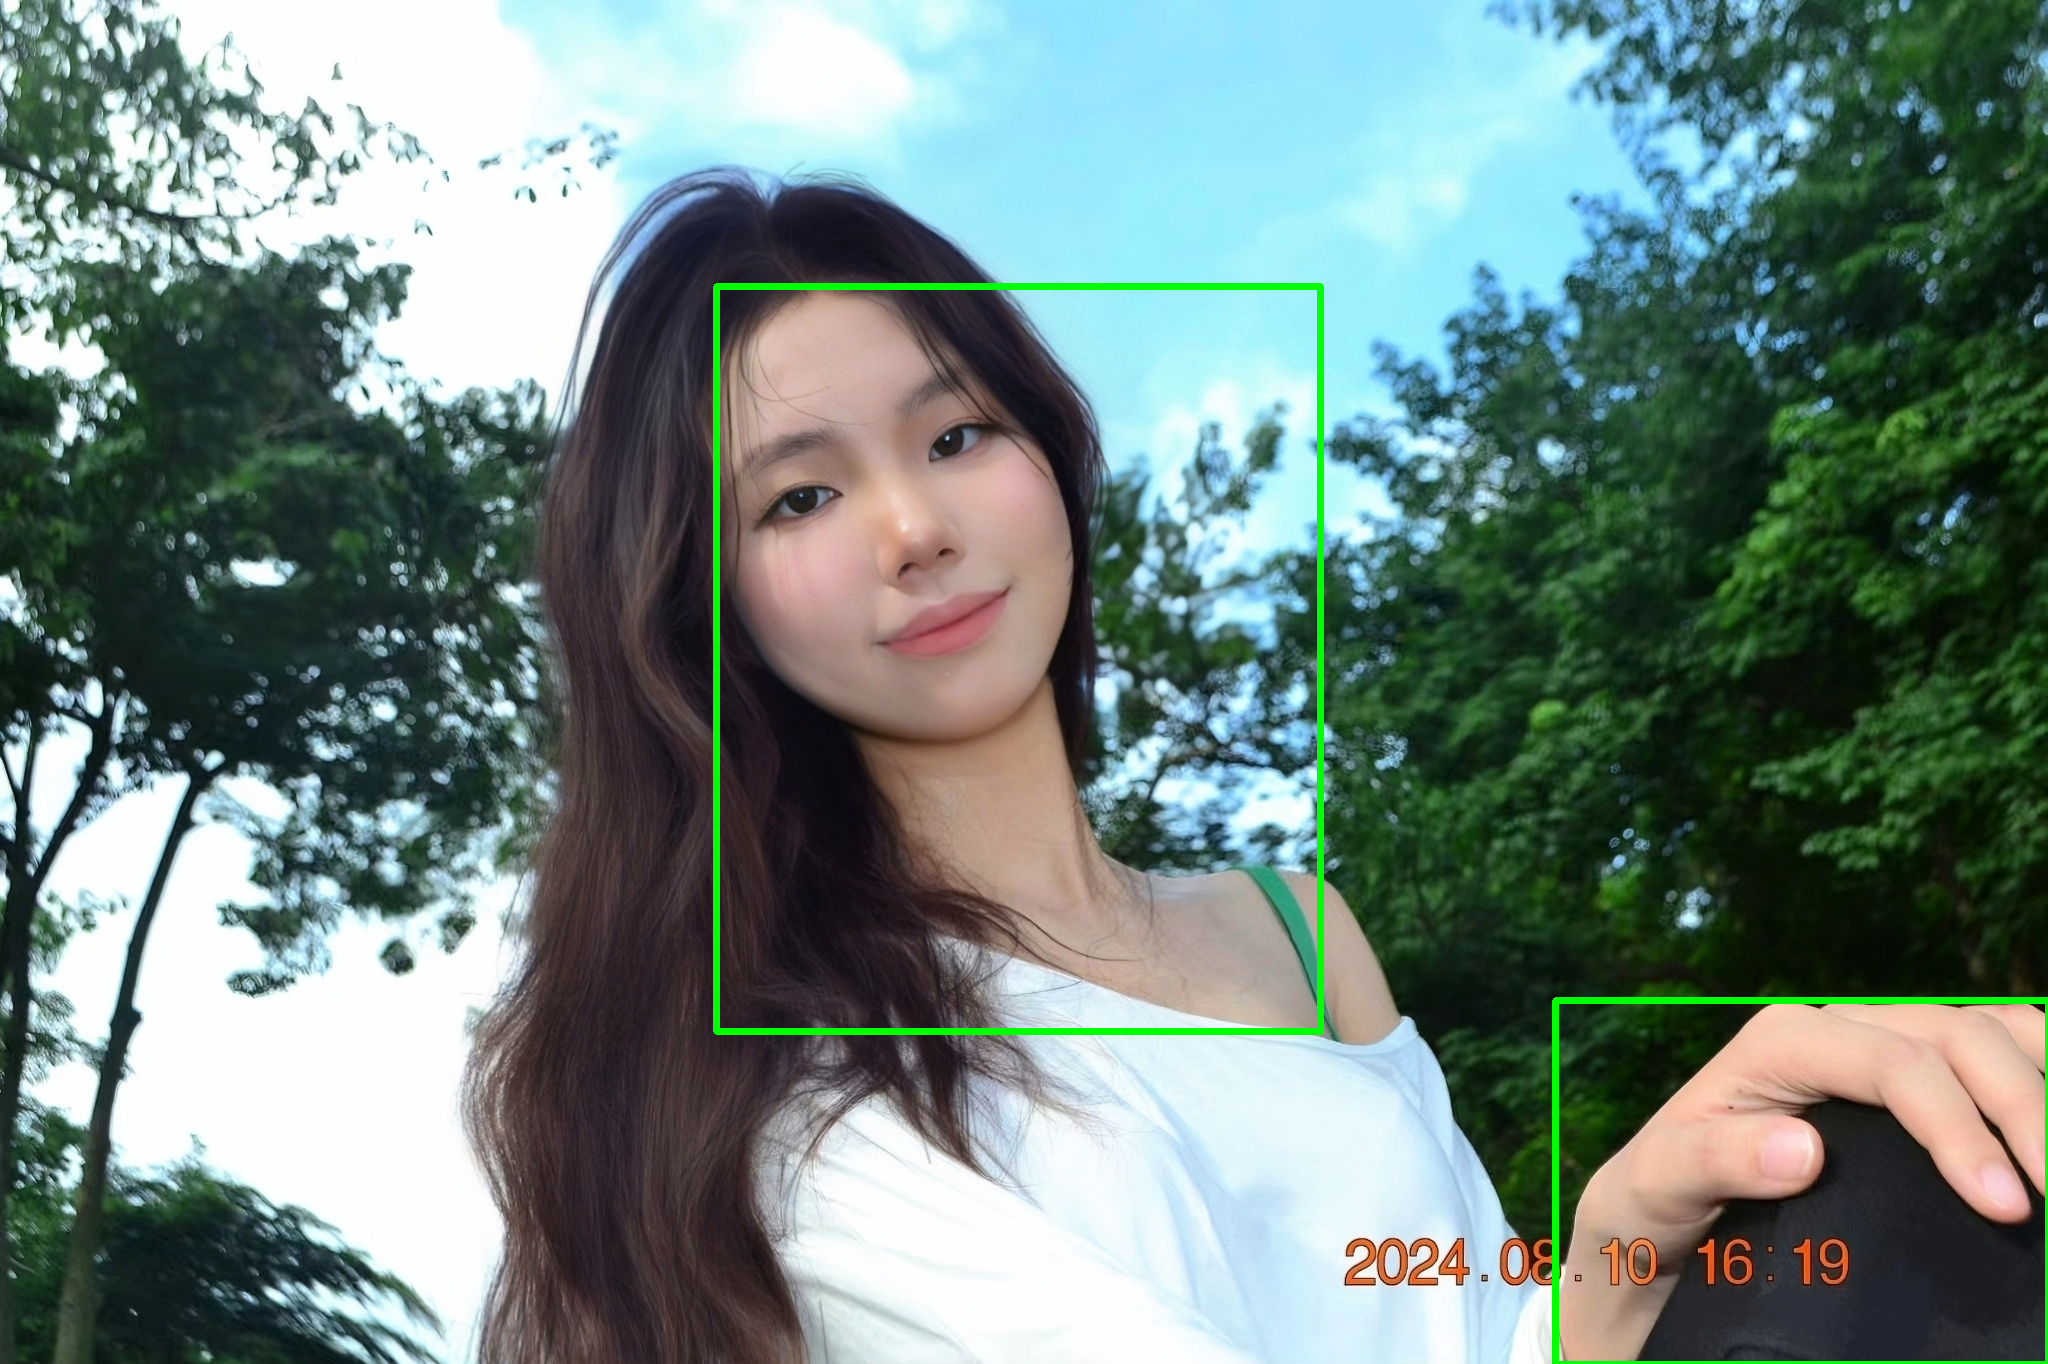
\includegraphics[height=.12\textheight]{./figure/color3.png}
		\end{subfigure}
		\caption{基于 YCgCr 颜色空间的人脸识别}
	\end{figure}
	
	在轻量化与高效性方面,Kim 等提出的 FeatherFace 方法,通过多层特征集成,兼顾检测精度与模型效率,在移动与嵌入式设备场景中具有良好表现\cite{mhfd2}。综述类研究如 Kumar 等则系统梳理了人脸检测领域的研究进展,指出当前挑战包括光照变化、姿态偏转、遮挡、多脸干扰以及肤色差异等,这些因素严重影响检测与识别精度​
	\cite{hfd}。
	
	在人脸识别过程中,高维图像数据往往引发“维度灾难”问题,传统降维技术如主成分分析(PCA)与线性判别分析(LDA)被广泛应用于特征提取与表示。Martinez 与 Kak 通过理论分析和实证对比指出,PCA 更擅长于保留样本的全局结构信息,而 LDA 能更有效地区分不同类别之间的差异,两者在特定应用场景中各具优势\cite{pcavslda}。Lu 等人基于 LDA 提出了多种改进的人脸识别算法,显著提升了小样本情形下的分类性能\cite{lda}。
	
	在分类方面,K 最近邻(KNN)作为一种非参数的监督学习方法,因其实现简单、适用于小样本问题的特点,在人脸识别任务中得到广泛使用。配合 PCA 或 LDA 进行降维后,KNN 可在低维空间中实现高效的最近邻查找,提高识别的精度与稳定性。此外,近年来部分研究尝试将 KNN 与核方法或距离加权策略结合,进一步提升其在边界模糊类间分布下的判别能力\cite{knn}。
	
	\section{方法}
	
	\subsection{PCA特征提取}
	
	主成分分析(Principal Component Analysis, PCA)是一种经典的线性降维技术,旨在从高维数据中提取最具代表性的低维特征。在人脸识别任务中,图像往往以高维向量表示,例如 $64 \times 64$ 的图像可被展平为 $4096$ 维的特征向量。如此高维的表示不仅带来了计算负担,也容易导致“维度灾难”,影响分类器性能。因此,采用 PCA 对图像数据进行降维处理,有助于去除冗余信息、降低噪声影响,并保留最具判别力的结构信息\cite{ml1, ml2, ml3, pca}。
	
	\begin{figure}[htbp]
		\centering
		\includegraphics[width=.8\textwidth]{./figure/PCAeigenfaces.png}
		\caption{PCA降维人脸示意图}
	\end{figure}
	
	PCA 的基本思路是通过正交线性变换,将原始样本映射到一组新的坐标轴上,使得新坐标轴上的各个分量互不相关,且按照数据方差从大到小排序。具体而言,设训练样本矩阵为 $X \in \mathbb{R}^{n \times d}$ ,其中 $n$ 是样本数,$d$ 是原始特征维度。首先对样本进行均值中心化,计算均值向量 $\mu = \frac{1}{n} \sum_{i=1}^n X_i$ ,然后构造协方差矩阵 $\Sigma = \frac{1}{n} (X-\mu)^T (X-\mu)$ 。通过对协方差矩阵进行特征值分解或奇异值分解,可以得到一组按方差大小排序的正交主成分向量。选取前 $k$ 个最大特征值对应的特征向量组成变换矩阵 $W \in \mathbb{R}^{d \times k}$ ,即可将原始样本投影到低维空间中,得到降维后的表示 $Z = (X-\mu)W$ 。
	
	在特征提取过程中,PCA 所保留的是数据在主轴方向上的最大方差,因此能较好地反映样本的整体结构分布。然而,由于 PCA 不依赖样本的类别标签,它在处理具有明显类间差异的人脸识别任务时,可能无法提供最优的判别能力。对此,后续我们引入基于监督信息的线性判别分析(LDA)方法进行对比分析\cite{pcavslda}。尽管如此,PCA 作为一种高效且无监督的特征压缩方法,仍在许多实际应用中表现出良好的性能,尤其在样本数量有限或数据存在较强共线性的情形下,其降维能力尤为显著。
	
	\begin{figure}[htbp]
		\centering
		\begin{minipage}{.45\textwidth}
			\centering
			\includegraphics[width=.8\textwidth]{./figure/PCAtrain.png}
			\caption{PCA二维训练集数据}
		\end{minipage}
		\begin{minipage}{.45\textwidth}
			\centering
			\includegraphics[width=.8\textwidth]{./figure/PCAtest.png}
			\caption{PCA二维测试集数据}
		\end{minipage}
	\end{figure}
	
	\subsection{LDA特征提取}
	
	线性判别分析(Linear Discriminant Analysis, LDA)是一种有监督的特征提取与降维方法,其核心目标在于通过类别标签的信息,最大化类间差异并最小化类内差异,从而在降维的同时增强样本的可判别性。在人脸识别任务中,LDA 以其优越的类别判别能力被广泛应用于特征提取阶段,特别是在面对高维、小样本的图像识别问题时,能够有效缓解“维数灾难”并提升识别精度\cite{ml1, ml2, ml3, lda}。
	
	\begin{figure}[htbp]
		\centering
		\includegraphics[width=.8\textwidth]{./figure/LDAeigenfaces.png}
		\caption{PCA降维人脸示意图}
	\end{figure}
	
	LDA 的基本思想是,在样本被映射到某一低维空间后,希望同类样本尽可能聚集,不同类样本之间尽可能分离。设样本矩阵为 $X \in \mathbb{R}^{n \times d}$ ,对应的类别标签为 $y \in \mathbb{R}^n$ ,其中 $n$ 为样本数,$d$ 为特征维度。首先需要计算所有样本的全局均值向量 $\mu = \frac{1}{n} \sum_{i=1}^n X_i$ ,然后按类别分别计算每一类的类内散度矩阵(within-class scatter matrix)与类间散度矩阵(between-class scatter matrix)。
	
	类内散度矩阵定义为:
	
	\vspace{-.5em}
	\begin{equation}
		S_w = \sum_{c=1}^C \sum_{x_i \in \mathcal{X}_c} (x_i - \mu_c)(x_i - \mu_c)^T
	\end{equation}
	 
	其中 $\mathcal{X}_c$ 表示第 $c$ 类的样本集合,$\mu_c$ 为该类的均值向量,$C$ 为类别数。
	
	类间散度矩阵定义为:
	
	\vspace{-.5em}
	\begin{equation}
		S_b = \sum_{c=1}^C n_c(\mu_c - \mu)(\mu_c - \mu)^T
	\end{equation}
	 
	其中 $n_c$ 为第 $c$ 类样本数量,$\mu$ 为全局均值向量。
	
	为了找到最优投影方向 $W$,LDA 通过最大化广义瑞利商(generalized Rayleigh quotient)来构建优化目标,即:
	
	\vspace{-.5em}
	\begin{equation}
		\max\limits_{W} \frac{\left| W^T S_b W \right|}{\left| W^T S_w W \right|}
	\end{equation}
	 
	其解对应于广义特征值问题:
	
	\vspace{-.5em}
	\begin{equation}
		S_b v = \lambda S_w v
	\end{equation}
	
	通过对 $S_w^{-1} S_b$ 进行特征值分解,选择前 $k$ 个最大特征值对应的特征向量组成投影矩阵 $W \in \mathbb{R}^{d \times k}$ ,即可将样本映射至 $k$ 维的线性判别子空间中,得到低维特征表示 $Z = XW$ 。
	
	\begin{figure}[htbp]
		\centering
		\begin{minipage}{.45\textwidth}
			\centering
			\includegraphics[width=.8\textwidth]{./figure/LDAtrain.png}
			\caption{LDA二维训练集数据}
		\end{minipage}
		\begin{minipage}{.45\textwidth}
			\centering
			\includegraphics[width=.8\textwidth]{./figure/LDAtest.png}
			\caption{LDA二维测试集数据}
		\end{minipage}
	\end{figure}
	
	需要注意的是,LDA 所能提取的最大特征维度为 $C-1$,其中 $C$ 是类别数。因此,当类别较少、原始维度又较高时,LDA 能有效实现维度压缩并增强类别判别性。与 PCA 相比,LDA 在降维过程中考虑了样本的类别信息,因而在监督学习场景下通常具有更强的分类性能\cite{pcavslda}。在本实验中,LDA 与 KNN 分类器结合使用,旨在评估其在人脸识别任务中的实际效能,并与 PCA 方法进行系统对比。
	
	\subsection{KNN分类器}
	
	K-最近邻(K-Nearest Neighbors, KNN)分类器是一种经典的非参数监督学习方法,其基本思想是在特征空间中根据样本之间的距离关系进行分类预测。KNN 不依赖于训练过程中的参数学习,而是将训练样本直接作为模型的一部分,待测试样本输入后,通过计算其与训练集中各样本之间的距离,选取最近的 $k$ 个邻居样本,根据多数投票原则决定测试样本的类别标签\cite{knn}。由于其原理简单、易于实现且具有良好的局部判别能力,KNN 广泛应用于图像识别、文本分类和推荐系统等领域\cite{ml1, ml2, ml3}。
	
	在本实验中,KNN 被用于对 PCA 或 LDA 提取后的低维特征进行分类识别。设训练样本特征集为 $\mathcal{D} = \{ (x_1, y_1), (x_2, y_2), ... , (x_n, y_n) \}$ ,其中 $x_i \in \mathbb{R}^d$ 为样本的低维特征向量,$y_i \in \{ 1, ... , C \}$ 表示类别标签。对于任意一个测试样本 $x \in \mathbb{R}^d$,KNN 通过计算其与训练样本的距离(通常使用欧氏距离):
	
	\vspace{-.5em}
	\begin{equation}
		d(x, x_i) = \left\| x-x_i \right\|_2 = \sqrt{\sum_{j=1}^d (x_j - x_{ij})^2}
	\end{equation}
	 
	获取与 $x$ 距离最近的 $k$ 个邻居样本集合 $\mathcal{N}_k(x)$,然后统计这些邻居样本中每个类别出现的频率,最终将 $x$ 预测为出现次数最多的类别:
	
	\vspace{-.5em}
	\begin{equation}
		\hat{y} = \arg \max\limits_{c \in \{ 1, ... , C \}} \sum_{x_i \in \mathcal{N}_k(x)} \mathbb{I}(y_i = c)
	\end{equation}
	
	其中 $\mathbb{I}(\ \cdot\ )$ 为指示函数,当括号内条件为真时返回 1,否则返回 0。
	
	KNN 分类器的性能主要受三个因素影响:一是特征空间的表示能力,这决定了距离度量的有效性;二是距离度量的选择,不同度量可能导致邻近关系差异较大;三是邻居数量 $k$ 的设定,较小的 $k$ 易受噪声干扰,较大的 $k$ 则可能掩盖局部特征。因此,在本实验中,我们结合 PCA 和 LDA 两种降维方式生成的特征空间进行比较,评估其在不同维度、不同邻居数 $k$ 下的分类准确率,以验证特征表示对 KNN 分类性能的影响。
	
	KNN 虽然不涉及参数训练,但在测试阶段需遍历全部训练样本,因此计算复杂度较高,尤其在高维空间中开销更为显著。因此结合降维方法对原始图像特征进行压缩,不仅有助于提高识别精度,也显著降低了 KNN 的运算成本\cite{ml1, ml2, ml3}。
	
	\section{实验}
	
	\subsection{基于KNN分类器的人脸识别}
	
	在本实验中,首先利用 PCA 和 LDA 方法分别对原始人脸图像数据进行降维,随后在降维后的特征空间中应用 K-最近邻(KNN)分类器完成人脸识别任务。为了保证特征在距离空间中的可比性,所有降维后的数据均经过标准化处理。KNN 分类器通过计算测试样本与训练样本之间的欧氏距离,选取距离最近的 $k=3$ 个邻居,并采用多数投票法进行分类预测。实验结果表明,在保留 8 个主成分的前提下,PCA 与 KNN 结合的识别准确率为 93.33\%,而 LDA 与 KNN 结合的识别准确率为 90.00\%。该结果说明,尽管 LDA 在理论上具有更强的类间可分性能力,但在当前特征维度和样本分布条件下,PCA 所保留的全局特征结构对 KNN 分类器的匹配性更好,可能更符合 Martinez 和 Kak 所指出的“当样本数较小时,PCA 往往比 LDA 更鲁棒”的结论\cite{pcavslda}。
	
	此外,由于 KNN 分类方法本身对局部样本结构高度敏感,其性能不仅依赖于特征空间的分布质量,也受到类别间边界清晰度的影响。因此在使用 LDA 降维后类别投影空间过于集中时,可能会降低 KNN 的判别性能。综上,KNN 在低维判别空间中表现出良好的分类能力,但仍需配合合适的特征表示策略以最大程度发挥其效果。
	
	\subsection{基于SVM分类器的人脸识别}
	
	为进一步验证降维特征在其他分类模型中的适应性,实验同时引入支持向量机(Support Vector Machine, SVM)作为替代分类器。SVM 通过构造最优间隔超平面实现二类或多类样本的判别,并在本实验中采用径向基函数(Radial Basis Function, RBF)核,以增强模型对非线性分布的适应能力。核函数的定义为 $K(x, x^{\prime})=\exp(-\gamma\left\|x-x^{\prime}\right\|^2)$,其中 $\gamma=0.1$,正则化参数 $C=10.0$。使用同样的 PCA 和 LDA 降维特征输入,训练 SVM 模型并在测试集上进行预测,最终结果显示:PCA + SVM 的识别准确率为 90.00\%,而 LDA + SVM 的识别准确率为 93.33\%。
	
	与 KNN 分类器的结果相比,SVM 在 LDA 特征空间中表现更优,说明其在处理类间差异高度集中的投影空间时具有更强的边界构建能力。由于 SVM 通过间隔最大化原则进行决策边界优化,因此在样本间距密集的 LDA 子空间中能够更有效地区分类别。此外,核函数的引入也提升了模型对复杂分布结构的表达能力,使得 LDA 降维后的特征在非线性分类器中具备更好的泛化效果。与之相比,PCA 降维后的特征保留了较多的全局变化趋势,但缺乏判别信息,使得在 SVM 中未能充分体现类别间边界的可分性。
	
	综上所述,KNN 和 SVM 两种分类器在不同特征表达方式下呈现出互补性:KNN 更适合于结构清晰、分布自然的 PCA 特征空间;而 SVM 在 LDA 构造的判别空间中则表现出更强的分类能力。这一结果不仅验证了不同降维策略与分类模型之间的协同效应,也印证了在实际人脸识别系统中需根据数据特性合理选择降维与分类方法的必要性。
	
	\section{结论}
	
	通过本次实验,我们系统地比较了基于 PCA 与 LDA 两种经典降维方法在人脸识别任务中的实际效果,并结合 K 最近邻(KNN)与支持向量机(SVM)两种常见分类器,对不同降维策略与分类模型的配合性能进行了分析。实验结果表明,不同降维方式在特征分布结构上具有明显差异,从而影响分类器的最终识别性能。在 KNN 分类器中,PCA 降维后的特征保留了更多原始数据的全局结构,表现出更高的准确率(93.33\%),相较之下,LDA 更倾向于将数据投影到紧凑的类间可分空间,但其在 KNN 上的性能略低(90.00\%)。而在 SVM 分类器中,这一趋势出现反转,LDA 与 SVM 的组合达到了最高识别率(93.33\%),明显优于 PCA 与 SVM(90.00\%),说明 LDA 提供的判别性特征更适合间隔优化型分类器。
	
	这些结果进一步印证了已有研究中对 PCA 与 LDA 特性差异的论断\cite{pcavslda}:PCA 更适合保持整体结构与全局变异性,适用于基于距离的分类模型;而 LDA 更注重类别间的判别性,因而在边界型或核方法分类器中效果更佳。此外,从整体趋势来看,不同降维方法与分类器之间存在明显的互补关系,说明在人脸识别系统中,算法组件的组合策略对于最终性能具有关键影响。
	
	未来的研究可以从以下几个方面展开:首先,考虑引入更多现代化的降维方法,如局部保持投影(LPP)、t-SNE 或 UMAP,与传统线性方法进行比较;其次,在分类器层面可尝试集成学习方法如随机森林或梯度提升树,以进一步提升鲁棒性与准确率;最后,面对更大规模、更多变的人脸数据,如何结合深度学习中的特征学习机制与传统降维技术构建轻量、可解释的人脸识别框架,是下一阶段值得深入探索的重要方向。本实验以对比分析为出发点,为进一步优化特征表达与分类模型选择提供了实验依据与方法参考。
	
	\let\cleardoublepage\clearpage
	
	\begin{thebibliography}{99}
		\bibitem{ml1} 谢文睿, 秦州, 贾彬彬. 机器学习公式详解[M]. 第2版. 北京:人民邮电出版社, 2023.
		\bibitem{ml2} 张伟楠, 赵寒烨, 俞勇. 动手学机器学习[M]. 第1版. 北京:人民邮电出版社, 2023.
		\bibitem{ml3} 周志华. 机器学习[M]. 第1版. 北京:清华大学出版社, 2016.
		\bibitem{pca} Abdi H, Williams L J. Principal component analysis[J]. Wiley interdisciplinary reviews: computational statistics, 2010, 2(4): 433-459.
		\bibitem{mhfd1} Alashbi A, Mohamed A H H M, El-Saleh A A, et al. Human face localization and detection in highly occluded unconstrained environments[J]. Engineering Science and Technology, an International Journal, 2025, 61: 101893.
		\bibitem{chfd1} De Dios J J, Garcia N. Face detection based on a new color space YCgCr[C]//Proceedings 2003 international conference on image processing (Cat. No. 03CH37429). IEEE, 2003, 3: III-909.
		\bibitem{chfd2} Ghazali K H B, Ma J, Xiao R. An innovative face detection based on YCgCr color space[J]. Physics Procedia, 2012, 25: 2116-2124.
		\bibitem{knn} Guo G, Wang H, Bell D, et al. KNN model-based approach in classification[C]//On The Move to Meaningful Internet Systems 2003: CoopIS, DOA, and ODBASE: OTM Confederated International Conferences, CoopIS, DOA, and ODBASE 2003, Catania, Sicily, Italy, November 3-7, 2003. Proceedings. Springer Berlin Heidelberg, 2003: 986-996.
		\bibitem{svm1} Hearst M A, Dumais S T, Osuna E, et al. Support vector machines[J]. IEEE Intelligent Systems and their applications, 1998, 13(4): 18-28.
		\bibitem{svm2} Jakkula V. Tutorial on support vector machine (svm)[J]. School of EECS, Washington State University, 2006, 37(2.5): 3.
		\bibitem{mhfd2} Kim D, Jung J, Kim J. FeatherFace: Robust and Lightweight Face Detection via Optimal Feature Integration[J]. Electronics, 2025, 14(3): 517.
		\bibitem{hfd} Kumar A, Kaur A, Kumar M. Face detection techniques: a review[J]. Artificial Intelligence Review, 2019, 52: 927-948.
		\bibitem{nhfd} Li H, Lin Z, Shen X, et al. A convolutional neural network cascade for face detection[C]//Proceedings of the IEEE conference on computer vision and pattern recognition. 2015: 5325-5334.
		\bibitem{lda} Lu J, Plataniotis K N, Venetsanopoulos A N. Face recognition using LDA-based algorithms[J]. IEEE Transactions on Neural networks, 2003, 14(1): 195-200.
		\bibitem{pcavslda} Martinez A M, Kak A C. Pca versus lda[J]. IEEE transactions on pattern analysis and machine intelligence, 2001, 23(2): 228-233.
		\bibitem{chfd3} Phung S L, Bouzerdoum A, Chai D. A novel skin color model in ycbcr color space and its application to human face detection[C]//Proceedings. International Conference on Image Processing. IEEE, 2002, 1: I-I.
	\end{thebibliography}
	
\end{document}
